\documentclass[12pt, titlepage]{article}

\usepackage{fullpage}
\usepackage[round]{natbib}
\usepackage{multirow}
\usepackage{booktabs}
\usepackage{longtable}
\usepackage{tabularx}
\usepackage{graphicx}
\usepackage{multirow}
\usepackage{float}
\usepackage[section]{placeins}
\usepackage{hyperref}
\hypersetup{
    colorlinks,
    citecolor=blue,
    filecolor=black,
    linkcolor=red,
    urlcolor=blue
}

%% Comments

\usepackage{color}

\newif\ifcomments\commentstrue %displays comments
%\newif\ifcomments\commentsfalse %so that comments do not display

\ifcomments
\newcommand{\authornote}[3]{\textcolor{#1}{[#3 ---#2]}}
\newcommand{\todo}[1]{\textcolor{red}{[TODO: #1]}}
\else
\newcommand{\authornote}[3]{}
\newcommand{\todo}[1]{}
\fi

\newcommand{\wss}[1]{\authornote{blue}{SS}{#1}} 
\newcommand{\plt}[1]{\authornote{magenta}{TPLT}{#1}} %For explanation of the template
\newcommand{\an}[1]{\authornote{cyan}{Author}{#1}}

%% Common Parts

\newcommand{\progname}{Sayyara Automotive Matcher} % PUT YOUR PROGRAM NAME HERE
\newcommand{\authname}{Team 27, Kappastone
\\ Tevis Doe, doet
\\ Caitlin Bridel, bridelc
\\ Gilbert Cherrie, cherrieg
\\ Rachel Johnson, johnsr12
\\ Harkeerat Kanwal, kanwalh
\\ Himanshu Aggarwal, aggarwah} % AUTHOR NAMES                  

\usepackage{hyperref}
    \hypersetup{colorlinks=true, linkcolor=blue, citecolor=blue, filecolor=blue,
                urlcolor=blue, unicode=false}
    \urlstyle{same}
                                


\newcounter{acnum}
\newcommand{\actheacnum}{AC\theacnum}
\newcommand{\acref}[1]{AC\ref{#1}}

\newcounter{ucnum}
\newcommand{\uctheucnum}{UC\theucnum}
\newcommand{\uref}[1]{UC\ref{#1}}

\newcounter{mnum}
\newcommand{\mthemnum}{M\themnum}
\newcommand{\mref}[1]{M\ref{#1}}

\begin{document}

\title{System Design for \progname{}} 
\author{\authname}
\date{\today}

\maketitle

\pagenumbering{roman}

\section{Revision History}

\begin{tabularx}{\textwidth}{p{3cm}p{2cm}X}
\toprule {\bf Date} & {\bf Version} & {\bf Notes}\\
\midrule
 Jan 18th, 2023 & 0.0 & Rev 0\\
\bottomrule
\end{tabularx}

\newpage

\section{Reference Material}

This section records information for easy reference.

\subsection{Abbreviations and Acronyms}

\renewcommand{\arraystretch}{1.2}
\begin{tabular}{l l} 
  \toprule		
  \textbf{symbol} & \textbf{description}\\
  \midrule 
  \progname & The application matches automotive owners with mechanics.\\
  FR & Functional Requirement \\
  PWA & Progressive Web App \\
  \bottomrule
\end{tabular}\\

\newpage

\tableofcontents

\newpage

\listoftables

\listoffigures

\newpage

\pagenumbering{arabic}

\section{Introduction}

This document will go over the design of the Sayyara Automotive Matcher. The document will give an overview of the design of the project, the design of the user interface, as well as give a timeline to the rest of the implementation of the project.

\section{Purpose}

The purpose of this document is to provide a more in depth look at the design, as well as provide more information to certain topics than previously covered in other documentation. The requirements outlined in the \href{https://github.com/HKanwal/kapstone/blob/main/docs/SRS/SRS.pdf}{SRS}
 will be linked to real design decisions made by the team in the implementation of the project. The timeline provided in the \href{https://github.com/HKanwal/kapstone/blob/main/docs/DevelopmentPlan/DevelopmentPlan.pdf}{Development Plan} will be made more concrete, outlining the rest of the implementation, the user testing that will be done, as well as the testing of the implementation outlined in the \href{https://github.com/HKanwal/kapstone/blob/main/docs/VnVPlan/VnVPlan.pdf}{VnV Plan}. By doing this, it is hoped that the document can provide a concrete outline of the design as well as how this design will be accomplished.

\section{Scope}
The system context described here was sourced from the SRS of this project.

\noindent 
\\The system context for the Sayyara Automotive Matcher is shown in Figure \ref{Fig_SystemContext}. This figure shows the relationship between the user inputs and the different parts of the software that the users interact with. The figure starts at the User box which shows the first stage of user input which is the user logging in as a customer, shop owner or shop employee. From this stage they are guided to the respective front end view of the PWA relevant to their access level and from these front end PWA views they have various interactions and user inputs that will interact with the database and have various outputs as shown by the arrows in the figure.

\begin{figure}[!Htb]
\centering
 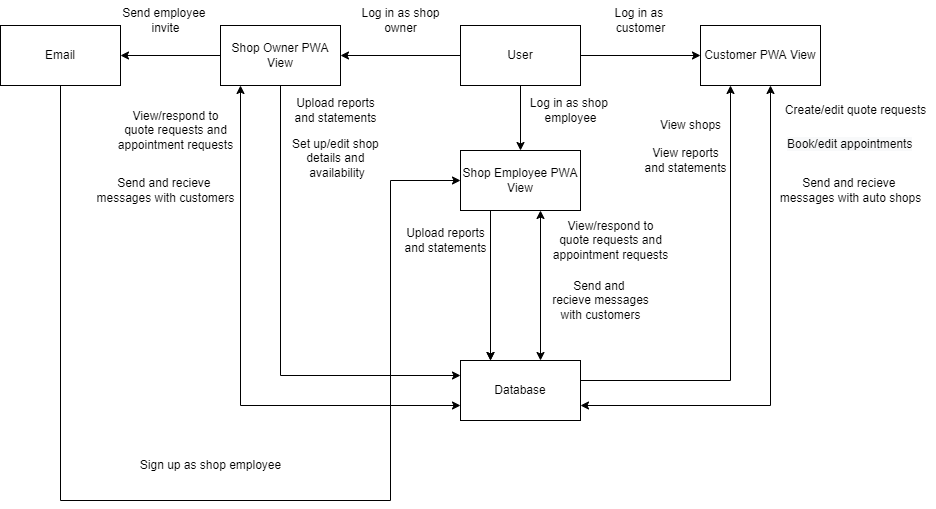
\includegraphics[width=1\textwidth]{SystemContext}
\caption{System context displaying user interactions with PWA views and database. }
\label{Fig_SystemContext} 
\end{figure}

\section{Project Overview}

\subsection{Normal Behaviour}

The Sayyara Automotive Matcher is an app that assists in communication between a mechanic and their potential customers. Customers are able to request quotes from different shops, receive said quotes from a shop, and finally schedule appointments with them. Shops will be able to manage the services that they provide to customers, manage the employees that work at the shop, manage appointments that they have scheduled, and provide quotes to prospective customers. Additionally, both customers and shops will be able to communicate with each other through a chat system.

\subsection{Undesired Event Handling}

The team will endeavor to minimize the amounts of undesired events as much as possible, however, they are inevitable, and so when an undesired event occurs, the team will follow these steps.

\begin{enumerate}
    \item 
    \item Present an error message to the user, and bar them from continuing.
    \begin{itemize}
        \item Preferably, this error message will be as specific as possible, using the user's terminology. Keep things simple.
        \item In the event of an unrecognized error, a generic error message will be used.
    \end{itemize}
    \item Identify the error on the team's side, using both the created test cases for the application, as well as viewing messages the app produces.
    \item Create a ticket the identifies the error as well as any relevant information to prevent it.
    \item If the undesired event is new, and as such uses a generic error message, first create a specific error message under another ticket, if the event requires one.
    \item Prevent the undesired event from occurring in the future, either by modifying the interface of the app, or by modifying the back-end to accept the event with no issue.
\end{enumerate}

By implementing an error message for the user, the team can keep the user more informed, and reduce frustration with the undesired event. Only after implementing a relevant error message will a fix be implemented.

\subsection{Component Diagram}

\noindent
The component diagram for the Sayyara Automotive Matcher is shown in Figure \ref{Fig_ComponentDiagram} This figure displays how the different user information interacts with the various front-end and back-end modules of the PWA as well as the interaction of the database module and database itself. All user types will interact with the Authentication, Account Creation, Quote Request, Quote, Appointment and Chat modules. The employee users can also interact with the work order module and the shop owners can also interact with the Shop Creation, Profile Page, Work Order and Employee modules. All these different front end modules will interact with the database module that submit and receive data from the database module which will send and receive data from the database. These interactions are all shown in the diagram through the arrows connecting the user information with the modules as well as the arrows connecting the front-end modules with the database modules to display the data and the direction it moves in.

\begin{figure}[H]
\centering
 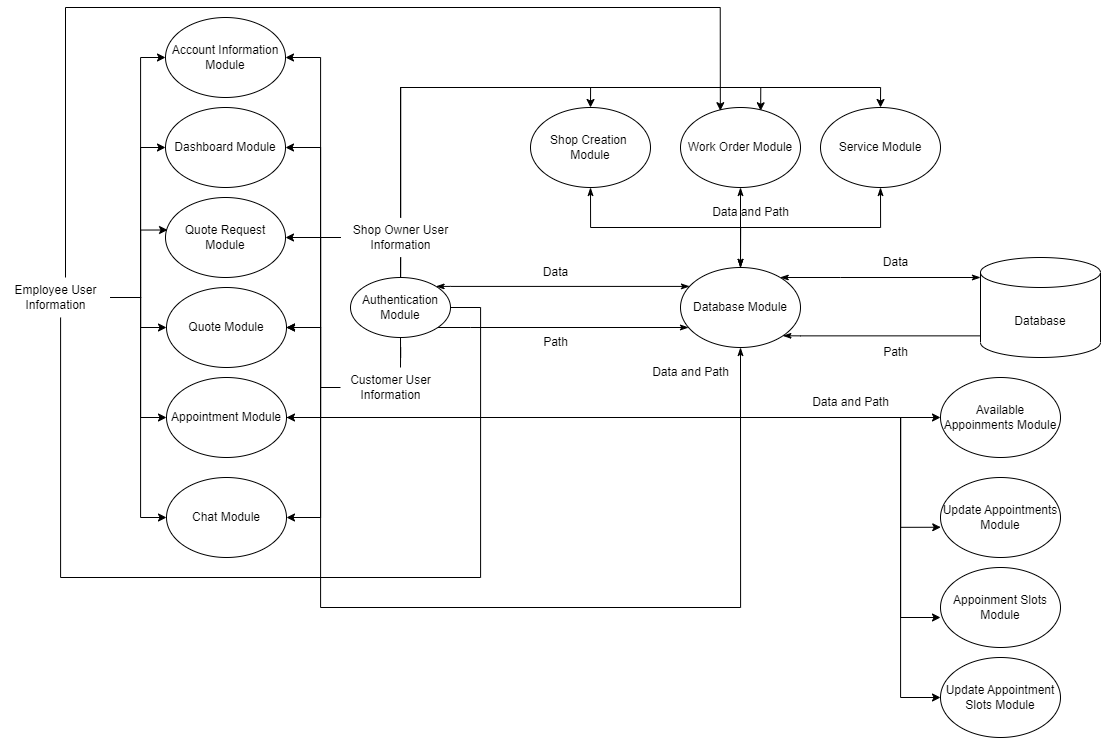
\includegraphics[width=1\textwidth]{ComponentDiagram.png}
\caption{Component diagram displaying the interaction between user information with the front-end and back-end modules.}
\label{Fig_ComponentDiagram} 
\end{figure}

\subsection{Connection Between Requirements and Design} \label{SecConnection}
For most of the functional requirements there exists a screen or page that was created to fulfill that requirement. 
\newline
To fulfill:
\newline
FR1: Created the shop registration page to allow shop owners to enroll their shop.
\newline
FR2, 4: Created the account creation page to allow shop owners and employees to create individual accounts.
\newline
FR3: Created employee invitation page to allow shop owners to send email invitations to employees.
\newline
FR5: Created the employee list page to view all employees and other users associated with the shop.
\newline
FR6: Added edit functionality to the account page to allow users to edit their accounts.
\newline
FR7: Added delete functionality to the account page to allow users to delete their accounts.
\newline
FR8: Created the login page to allow shop owners, employees and customers to login to their accounts using a username and password.
\newline
FR9: Added forgot password functionality to the login page to allow users to reset their password.
\newline
FR10, 11: Created the quote response page to allow shop owners and employees to create quotes and send them to customers.
\newline
FR12: Created the shop appointment page to allow shop owners and employees to accept or reject an appointment submitted by a customer.
\newline
FR14: Created the employee list page to allow shop owners view, search for, and filter all employees as well as add and remove employees.
\newline
FR15, 16: Created the work order page to allow shop owners and employees to create work orders and send them to customers.
\newline
FR17, 19: Added edit functionality to the shop profile page to allow shop owners to edit their shop profile and set shop availability.
\newline
FR20, 30: Created the shop search screen that users can access without an account to allow all customers to search for and filter shops and view shop profiles.
\newline
FR21: Added functionality for customers to submit rework requests through the quote screen to allow for customer rework requests.
\newline
FR22: Created the submitted quote request list screen to allow shop owners and employees to view, search for, and filter quote requests.
\newline
FR23: Created the work order list screen to allow shop owners and employees to view, search for, and filter work orders.
\newline
FR24: Created the chat functionality to allow customers to chat with shop owners and employees.
\newline
FR25: Added back-end functionality that will automatically delete a work order if the appointment is cancelled.
\newline
FR26: Added back-end functionality that will automatically create a work order if an appointment is created.
\newline
FR27: Added functionality to the work order page to allow shop owners and employees to assign work orders to employees.
\newline
FR28: Created the appointment page to allow customers to book appointments.
\newline
FR29: Created the quote request page to allow customers to submit quote requests.

\section{User Interfaces}

\noindent
The design of the user interface was created as a group using Figma, which is linked in Appendix A. The design of the user interface was created in order to meet all the functionality requirements presented by our supervisor. The overall design is separated into two sections, one which is the customer view and another which is for the shop owner or employee view. These separate views allowed us to break down which pages would be needed for each user type and the information that would be required for each page. Each page was created in order to fulfill some functional requirement and then within each page we worked to design a user interface that would be easy to use and intuitive. In order to make the design intuitive we relied on common design features found in other mobile apps so that users can leverage previous knowledge and information to use our application easier. We also made sure that the pages and overall design presented all information clearly, made user interaction efficient and only included what was necessary without including any extra pages or features that could overwhelm and confuse the user. This all allows for a very streamlined design that aids in allowing the app to be easy to use.

\section{Timeline}

Time-spans generally are given in roughly two week periods, as those are the length of the sprints the team uses. \\

\begin{longtable}{ p{3cm}p{3.5cm}p{5cm}p{3cm}  }
 \hline
 \textbf{Task} & \textbf{Time-span} & \textbf{Description} & \textbf{Responsible Person(s)} \\
 \hline
 Design documents & Jan. 4 - Jan. 18 & Design documents as specified by the course. & Whole Team \\
 \hline
 Complete Quote Request implementation & Jan. 17 - Jan. 31 & Fully implement quote request functionality. Changes on both the quote request screens on the front-end and in the back-end representation of quote requests must be made. & Tevis, Gilbert, Rachel \\
 \hline
 Complete Quote implementation & Jan. 17 - Jan. 31 & Fully implement quote functionality. Both front-end and back-end are almost fully capable in coordinating this, but some changes still must be made. & Tevis, Gilbert \\
 \hline
 Shop profile page & Jan. 17 - Jan. 31 & Profile page for shop owners. & Himanshu \\
 \hline
 Appointment Scheduling & Jan. 17 - Jan. 31 & Enable customers to book appointments with shops through the interface. May bleed into next sprint as needed. & Himanshu, Harkeerat \\
 \hline
  Completion of User Interface, full implementation & Jan. 31 - Rev. 0 Demo & Complete any remaining tasks as required for the revision 0 demo.  Likely tasks:
    \begin{itemize}
        \item Find Shop screen
        \item User image display in app
        
    \end{itemize}
& Whole Team \\
 \hline
  NextJS Testing & Jan. 31 - Rev. 0 Demo & Implement tests regarding NextJS as detailed in the VnV Plan & Gilbert, Rachel, Harkeerat \\
 \hline
 Django Testing & Jan. 31 - Rev. 0 Demo & Implement tests regarding Django as detailed in the VnV Plan & Tevis, Himanshu \\
 \hline
  User Testing & Feb. 21 - Mar. 7 & After Rev. 0 demo, gather feedback from users about the interface, functionality, etc. Draft changes into tickets that are actionable. & Tevis, Rachel \\
 \hline
   User Testing Feedback Implementation & Feb. 21 - Final Demo & Implement ideas gotten from user testing as they come up. We hope to spend at least 2 weeks on this. & Whole Team \\
 \hline
 VnV Report & Feb. 21 - Mar. 7 & Complete the VnV report as specified by the course. & Whole Team \\
 \hline
 Revision 1 Cleanup & Mar. 7 - Final Demo & Address any issues with the project, implement any missing features, gain confidence in the implementation. & Whole Team \\
 \hline
 Documentation Revision 1 & Mar. 21 - April 5 & Revise documentation to fit the current state of the project. & Whole Team \\
 \hline
 
\end{longtable}

% \bibliographystyle {plainnat}
% \bibliography{../../../refs/References}

\newpage{}

\appendix

\section{Interface}


[1] \href{https://www.figma.com/file/TsSCB9xRZcJgC8ZJnOhxEm/Sayyara-Automotive-Matcher-w\%2F-Template?node-id=6690\%3A116&t=meQ7BcozE7pEMGGX-1}{Figma}
\section{Mechanical Hardware}

\section{Electrical Components}

\section{Communication Protocols}

\section{Reflection}

The information in this section will be used to evaluate the team members on the
graduate attribute of Problem Analysis and Design.  Please answer the following questions:

\begin{enumerate}
  \item What are the limitations of your solution?  Put another way, given
  unlimited resources, what could you do to make the project better? (LO\_ProbSolutions)
  
  If given unlimited resources we could make the project better by essentially fully implementing all features that our supervisor has given us. This includes the features indicated as required for the minimal viable product as well as features listed as nice to have or optional. Also, we would work to further improve non-functional requirements of the product so they are not only meeting the minimal criteria but further improving them to surpass all the criteria until they can no longer be improved. Also, we would work on the product to ensure it is scalable both on the front-end by making new features easy to add and on the back-end by making the back-end much more scalable to be able to support as many users and data as possible.
  
  \item Give a brief overview of other design solutions you considered.  What
  are the benefits and tradeoffs of those other designs compared with the chosen
  design?  From all the potential options, why did you select documented design?
  (LO\_Explores)
  
  The solutions that we considered were mostly similar, as the team had the design constraint of developing a PWA, as dictated via our supervisor, however we did make a few designs within that constraint. At first, the team created a design that was made for desktop first. Our thoughts were to make a design and then reduce it for a mobile version. By doing this, we could work with what the team was more familiar with, desktop environments, and then create a mobile version based off of it. Unfortunately, this did not work out for us, as the desktop version of our design could not be reduced to a mobile version without creating too many changes. We realized that our implementation needed to be common, or else we were just going to end up building 2 different apps, which is against a PWAs design principles. Our next design was an initial mobile design. It was our hope that we could just expand the mobile design into a desktop version with little to no issue. Unfortunately, somewhere along the way, we ended up with something a bit too minimalist. Not enough information was provided to the user to navigate through the application comfortably, and overall it didn't translate very well to the desktop version either. The second design certainly looked prettier than our current one, but we could not use it. Our third, and final design was one that made concessions. It looked worse than the second design, but provided the relevant information to a user in an easy way. It didn't fit as well on the desktop as the first design, however it could work on both the desktop and mobile comfortably. These concessions are why we made it our documented design.
\end{enumerate}

\end{document}